\section{Dynamical Core}\label{sec:dyncore}

In this section we describe the dynamical core of ECHAM. The first two sections present the governing equations,
the coordinates and the discretization schemes used. Attention is
concentrated on the representation of the explicitly resolved
adiabatic processes. A derivation of the equations including terms
requiring parameterization is included in Appendix \ref{sec:diabat}.

The dynamical part of ECHAM is formulated in spherical
harmonics. After the inter-model comparisons by \cite{jarraud81} and
\cite{girard82} truncated expansions in terms of spherical harmonics
were adopted for the representation of dynamical fields. The transform
technique developed by \cite{eliasen70}, \cite{orszag70}, and
\cite{machenhauer72} is used such that non-linear terms, including
parameterizations, are evaluated at a set of almost regularly
distributed grid points - the Gaussian grid.

In the vertical, a flexible coordinate is used, enabling the model to
use either the usual terrain-following sigma coordinate
\cite[]{phillips57}, or a hybrid coordinate for which upper-level model
surfaces flatten over steep terrain, becoming surfaces of constant
pressure in the stratosphere (\cite{simmons81a} and
\cite{simmons81b}). Moist processes are treated in a different way using 
a mass conserving algorithm for the transport \cite[]{lin96} of the
different water species and potential chemical tracers. The transport
is determined on the Gaussian grid.

First, in section \ref{sec:contequ} the continuous form of the
governing equations is presented. Sections \ref{sec:hordis} and
\ref{sec:verdis} give details of the spectral representation and of
the vertical coordinate and its associated vertical finite difference
scheme. The temporal finite-difference scheme, which includes not only
a conventional semi-implicit treatment of gravity-wave terms
\cite[]{robert72}, but also a semi-implicit treatment of the advection
of vorticity \cite[]{jarraud82}, is described in section
\ref{sec:timdis}.

\subsection{\label{sec:contequ}The continuous equations} 

Although the model has been implemented for one particular form of a
vertical coordinate, which is introduced in section \ref{sec:verdis},
it is convenient to introduce the equations and their spectral
representation for a general pressure-based terrain-following vertical
coordinate $\eta(p,p_s)$, which must be a monotonic function of
pressure $p$, and depends as well on the surface pressure $p_s$, in
such a way that

\[
\eta(0,p_s) = 0 \qquad \mbox{and} \qquad \eta(p_s,p_s) = 1
\]

For such a coordinate, the continuous formulation of the primitive
equations for a dry atmosphere may be directly derived from their
basic height coordinate forms following \cite{kasahara74}.

During the design of the model, a detailed derivation of the
corresponding equations for a moist atmosphere, including a separation
into terms to be represented explicitly in the subsequent discretized
form of the equations and terms to be parameterized, was carried
out. It is shown in Appendix \ref{sec:diabat} that under certain
approximations, the momentum, thermodynamic and moisture equations may
be written:

\begin{eqnarray}
\dnd{U}{t}-(f+\xi)V+\dot{\eta}\dnd{U}{\eta}+\frac{R_dT_v}{a}
  \dnd{\ln{p}}{\lambda}+\frac{1}{a}\dnd{(\phi+E)}{\lambda} 
& = & P_U+K_U
\label{(2.2.1)}
\\
\dnd{V}{t} +(f+\xi)U+\dot{\eta}\dnd{V}{\eta}+\frac{R_dT_v}{a}(1-\mu^2)
\dnd{\ln{p}}{\mu}+\frac{(1-\mu^2)}{a}\dnd{(\phi+E)}{\mu} 
& = & P_V+K_V
\label{(2.2.2)}
\\ 
\dnd{T}{t} +\frac{U}{a(1-\mu^2)}\dnd{T}{\lambda}+\frac{V}{a}\dnd{T}{\mu}
+\dot{\eta}\dnd{T}{\eta}-\frac{\kappa T_v\omega}{(1+(\delta-1)q_v)p}
& = & P_T+K_T
\label{(2.2.3)}
\\ 
\dnd{q_i}{t}+\frac{U}{a(1-\mu^2)}\dnd{q_i}{\lambda}+\frac{V}{a}\dnd{q_i}{\mu}
+\dot{\eta}\dnd{q_i}{\eta}
& = & P_{q_i}
\label{(2.2.4)}
\end{eqnarray}

where $q_i$ are the mixing ratios of the different water species.

The continuity equation is

\begin{equation}
\dnd{}{\eta}\left(\dnd{p}{t}\right)+\nabla\cdot\left(\vec{v}_h\dnd{p}{\eta}\right)
+\dnd{}{\eta}\left({\dot{\eta}}\dnd{p}{\eta}\right) = 0
\label{(2.2.6)} 
\end{equation}

and the hydrostatic equation takes the form

\begin{equation}
\dnd{\phi}{\eta} = -\frac{R_dT_v}{p}\dnd{p}{\eta}
\label{(2.2.7)} 
\end{equation}
The pressure coordinate vertical velocity is given by

\begin{equation}
\omega = \vec{v}_h\nabla p
-\int\limits_0^{\eta}\nabla\cdot\left(\vec{v}_h\dnd{p}{\eta}\right) d\eta
\label{(2.2.8)} 
\end{equation}

and explicit expressions for the rate of change of surface pressure,
and for $\dot{\eta}$, are obtained by integrating equation
\ref{(2.2.6)}, using the boundary conditions $\dot{\eta} = 0$ at $\eta
= 0$ and $\eta = 1$:

\begin{equation}
\dnd{p_s}{t} = -\int\limits_0^1 \nabla\cdot\left(\vec{v}_h\dnd{p}{\eta}\right) d\eta
\label{(2.2.9)} 
\end{equation}

and

\begin{equation}
\dot{\eta}\dnd{p}{\eta} = -\dnd{p}{t}-\int\limits_0^{\eta}
\nabla\cdot\left(\vec{v}_h\dnd{p}{\eta}\right) d\eta
\label{(2.2.10)}
\end{equation} 

equation \ref{(2.2.9)} may also be written

\begin{equation}
\dnd{\ln{p_s}}{t} = -\frac{1}{p_s}\int\limits_0^1 
\nabla\cdot\left(\vec{v}_h\dnd{p}{\eta}\right) d\eta
\label{(2.2.11)}
\end{equation}

Following the derivation given in Appendix \ref{sec:diabat}, the terms
$P_U$, $P_V$, $P_T$, and $P_{q_i}$ are written:

\begin{eqnarray}
P_U & = &  -g\cos{\theta}\left(\dnd{p}{\eta}\right)^{-1}\dnd{J_U}{\eta}
\label{(2.2.12)} \\
P_V & = &  -g\cos{\theta}\left(\dnd{p}{\eta}\right)^{-1}\dnd{J_V}{\eta}
\label{(2.2.13)} \\  
P_T & = &  \frac{1}{c_p}\left[Q_R+Q_L+Q_D-g\left(\dnd{p}{\eta}\right)^{-1}
\left(\dnd{J_S}{\eta}-c_{pd}T(\delta-1)\dnd{J_{q_v}}{\eta}\right)\right]
\label{(2.2.14)} \\
P_{q_i} & = & S_{q_i} -g\left(\dnd{p}{\eta}\right)^{-1}\dnd{J_{q_i}}{\eta}
\label{(2.2.15)} 
\end{eqnarray}

where

\[
c_p = c_{pd}(1+(\delta-1)q_v)
\]	

In equations \ref{(2.2.12)} - \ref{(2.2.15)}, $J_U$, $J_V$, $J_S$, and
$J_{q_i}$ represent net parameterized vertical fluxes of momentum, dry
static energy $(c_pT+\phi)$, moisture and cloud species. They include
fluxes due to convection and boundary-layer turbulence. $Q_R$, $Q_L$,
and $Q_D$ represent heating due to radiation, phase changes
and to internal
dissipation of kinetic energy associated with the $P_U$ and $P_V$
terms, respectively. $S_{q_i}$ denotes the rates of change of $q_i$
due to phase changes and precipitation formation. Details
of the calculation of these terms are given in section
\ref{sec:cloud}.

The $K$ terms in equations \ref{(2.2.1)} - \ref{(2.2.4)} represent the
influence of unresolved horizontal scales. Their treatment differs
from that of the $P$ terms in that it does not involve a physical model of
sub-grid scale processes, but rather a numerically convenient form of
scale selective diffusion of a magnitude determined empirically to
ensure a realistic behaviour of resolved scales.
% These terms are specified in section \ref{sec:hordif}.

In order to apply the spectral method, equations \ref{(2.2.1)} and
\ref{(2.2.2)} are written in vorticity and divergence form following
\cite{bourke72}. They become

\begin{eqnarray}
\dnd{\xi}{t} & = & \frac{1}{a(1-\mu^2)}\dnd{(F_V+P_V)}{\lambda}
-\frac{1}{a}\dnd{(F_U+P_U)}{\mu}+K_{\xi}
\label{(2.2.17)}\\
\dnd{D}{t}   & = & \frac{1}{a(1-\mu^2)}\dnd{(F_U+P_U)}{\lambda}
+\frac{1}{a}\dnd{(F_V+P_V)}{\mu}-\nabla^2G+K_D
\label{(2.2.18)} 
\end{eqnarray}

where

\begin{eqnarray}
F_U & = & (f+\xi)V-\dot{\eta}\dnd{U}{\eta}
         -\frac{R_dT_v}{a}\dnd{\ln{p}}{\lambda}
\label{(2.2.19)}\\
F_V & = & -(f+\xi)U-\dot{\eta}\dnd{V}{\eta}
         -\frac{R_dT_v}{a}(1-\mu^2)\dnd{\ln{p}}{\lambda}
\label{(2.2.20)} 
\end{eqnarray}

and

\begin{equation}
G = \phi+E
\label{(2.2.21)} 
\end{equation}

We also note that a streamfunction $\psi$ and velocity potential
$\chi$ may be introduced such that

\begin{eqnarray}
U & = & \frac{1}{a}\left[-(1-\mu^2)\dnd{\psi}{\mu}+\dnd{\chi}{\lambda}\right]
\nonumber\\
V & = & \frac{1}{a}\left[\dnd{\psi}{\lambda}+(1-\mu^2)\dnd{\chi}{\mu}\right]
\label{(2.2.22)}
\end{eqnarray}

and

\begin{eqnarray}
\xi & = & \nabla^2\psi \nonumber\\
D   & = & \nabla^2\chi
\label{(2.2.22a)}
\end{eqnarray}

\subsection{\label{sec:hordis}Horizontal discretization}

\subsubsection{Spectral representation} 

The basic prognostic variables of the model are $\xi$, $D$, $T$,
$q_i$, and $\ln p_s$. While $q_i$ are represented in grid point space,
the other variables, and the surface geopotential $\phi_s$, are
represented in the horizontal by truncated series of spherical
harmonics:

\begin{equation}
X(\lambda,\mu,\eta,t) = \sum\limits_{m = -M}^M \sum\limits_{n=m}^{N(M)}
X_n^m(\eta,t) P_n^m(\mu)\e{im\lambda}
\label{(2.3.1.1)} 
\end{equation}

where $X$ is any variable, $m$ is the zonal wave number and $n$ is the
meridional index. The $P_n^m$ are the Associated Legendre Functions of the
first kind, defined here by

\begin{equation}
P_n^m(\mu) = \sqrt{(2n+1)\frac{(n-m)!}{(n+m)!}}\,\frac{1}{2^nn!}
(1-\mu^2)^{\frac{m}{2}} \frac{d^{(n+m)}}{d\mu^{(n+m)}}(\mu^2-1)^n, 
\quad (m \ge 0)
\label{(2.3.1.2)}
\end{equation}

and

\[
P_n^{-m}(\mu) = P_n^m(\mu)
\]

This definition is such that

\begin{equation}
\frac{1}{2} \int\limits_{-1}^1 P_n^m(\mu)P_s^m(\mu) d\mu = \delta_{ns}
\label{(2.3.1.3)}
\end{equation}

where $\delta_{ns}$ is the Kronecker delta function. The $X_n^m$ are
the complex-valued spectral coefficients of the field $X$ and given by

\begin{equation}
X_n^m(\eta,t) = \frac{1}{4\pi}\int\limits_{-1}^1\int\limits_0^{2\pi}
X(\lambda,\mu,\eta,t) P_n^m(\mu) \e{-im\lambda} d\lambda d\mu
\label{(2.3.1.4)} 
\end{equation}

Since $X$ is real

\begin{equation}
X_n^{-m} = (X_n^m)^*
\label{(2.3.1.5)}
\end{equation}

is valid, where $(\;)^*$ denotes the complex conjugate. The model thus
deals explicitly only with the $X_n^m$ for $m \ge 0$. 

The Fourier coefficients of $X$, $X_m(\mu,\eta,t)$ are defined by

\begin{equation}
X_m(\mu,\eta,t) = \frac{1}{2\pi}\int\limits_0^{2\pi}
X(\lambda,\mu,\eta,t)\e{-im\lambda} d\lambda
\label{(2.3.1.6)} 
\end{equation}

or, using equation \ref{(2.3.1.1)}, by

\begin{equation}
X_m(\mu,\eta,t) = \sum\limits_{n=m}^{N(m)} X_n^m(\eta,t) P_n^m(\mu)
\label{(2.3.1.7)}
\end{equation}

with

\begin{equation}
X(\lambda,\mu,\eta,t) = \sum\limits_{m = -M}^M 
X_m(\mu,\eta,t) \e{im\lambda}
\label{(2.3.1.8)} 
\end{equation}

Horizontal derivatives are given analytically by

\begin{equation}
\left(\dnd{X}{\lambda}\right)_m = imX_m
\quad \mbox{and} \quad
\left(\dnd{X}{\mu}\right)_m = \sum\limits_{n=m}^{N(m)} X_n^m 
\frac{dP_n^m}{d\mu}
\label{(2.3.1.9)}
\end{equation}

where the derivative of the Legendre Function is given by
the recurrence relation:

\begin{equation}
(1-\mu^2)\frac{dP_n^m}{d\mu} = -n\varepsilon_{n+1}^mP_{n+1}^m+(n+1)
\varepsilon_n^mP_{n-1}^m
\quad \mbox{with} \quad
\varepsilon_n^m = \sqrt{\frac{n^2-m^2}{4n^2-1}}
\label{(2.3.1.11)} 
\end{equation}

An important property of the spherical harmonics is the algebraic form
of the Laplacian:

\begin{equation}
\nabla^2(P_n^m(\mu)\e{im\lambda}) = -\frac{n(n+1)}{a^2}P_n^m(\mu)\e{im\lambda}
\label{(2.3.1.13)}
\end{equation}

Relationships \ref{(2.2.22)} and \ref{(2.2.22a)} may thus be used to
derive expressions for the Fourier velocity coefficients, $U_m$ and
$V_m$ in terms of the spectral coefficients $\xi^m_n$ and $D^m_n$. It
is convenient for later reference to write these expressions in the
form

\begin{equation}
U_m = U_{\xi m} + U_{Dm} \quad \mbox{and} \quad V_m = V_{\xi m} + V_{Dm} 
\label{(2.3.1.14)} 
\end{equation}

where

\begin{eqnarray}
U_{\xi m} & = & -a\sum\limits_{n=m}^{N(m)}\frac{1}{n(n+1)}  \xi_n^mH_n^m(\mu)\\
U_{Dm}    & = & -a\sum\limits_{n=m}^{N(m)}\frac{im}{n(n+1)} D_n^mP_n^m(\mu)\\
V_{\xi m} & = & -a\sum\limits_{n=m}^{N(m)}\frac{im}{n(n+1)} \xi_n^mP_n^m(\mu)\\
V_{Dm}    & = & -a\sum\limits_{n=m}^{N(m)}\frac{1}{n(n+1)}  D_n^mH_n^m(\mu)
\label{(2.3.1.19)}
\end{eqnarray}

with

\begin{equation}
H_n^m(\mu) = -(1-\mu^2)\frac{dP_n^m}{d\mu}
\label{(2.3.1.20)}
\end{equation}

The $H_n^m$ can be computed from the recurrence relation
\ref{(2.3.1.11)}. In \echam{} only triangular truncations can be used
which is the preferred type of truncations for resolutions larger than
T31. This restriction is implied by the parallelization of the
spectral part of the model. The triangular truncation is completely
defined by the three parameters illustrated in figure
\ref{fig:triangular}.

\begin{figure}[htb]
\[
\ifpdf
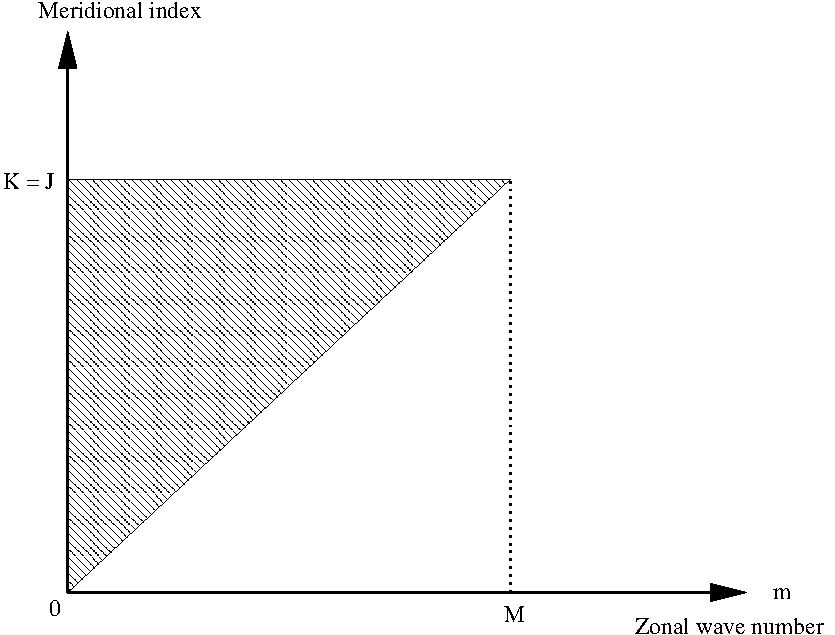
\includegraphics[width=0.6\linewidth]{science/triangular.pdf}
\else
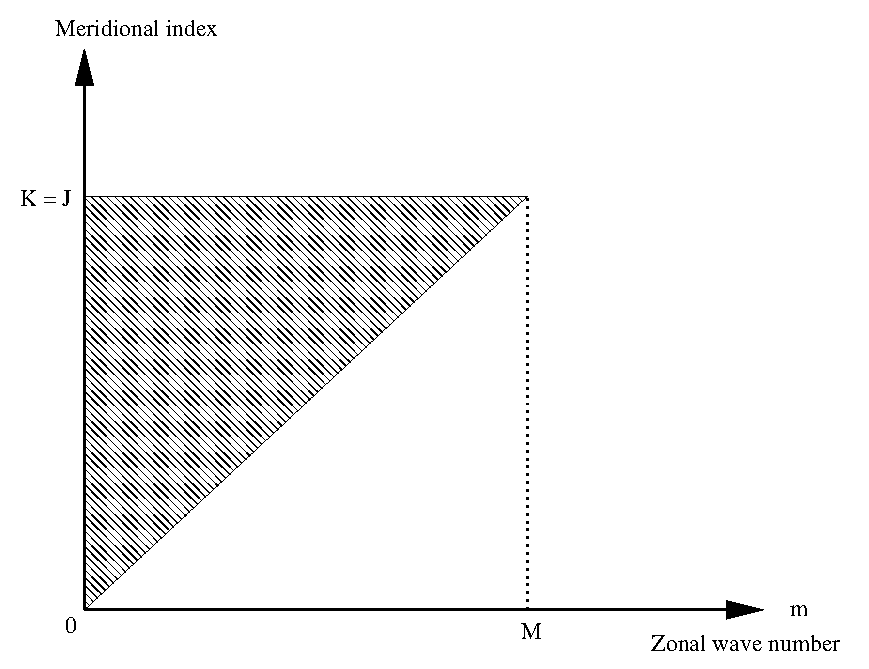
\includegraphics{science/triangular.eps}
\fi
\]
\caption{\label{fig:triangular}Triangular truncation}
\end{figure}

The triangular truncations are special cases of the pentagonal one in which
$M = J = K$.  

The summation limit, $N(m)$ is given by
\[
N = J+|m| \qquad \mbox{if} \qquad J+|m| \le K \qquad
\mbox{and} \qquad
N = K \qquad \mbox{if} \qquad J+|m| > K
\]

The standard truncations used in \echam{} are at wave numbers 31,
63, 127 or 255.

\clearpage

\subsubsection{Spectral/grid-point transforms, and the evaluation of 
               spectral tendencies} 

The general form of the equations follow that of the early multi-level
spectral models described by \cite{bourke74} and \cite{hoskins75},
although the present model differs in its use of an advective form for
the equations \ref{(2.2.17)}, \ref{(2.2.18)}, \ref{(2.2.3)}, and
\ref{(2.2.11)}. Equations for the corresponding spectral coefficients
are obtained by multiplying each side of these equations by
$P^m_n(\mu)\e{-im\lambda}$ and integrating over the sphere. This
yields, from \ref{(2.3.1.4)},

\begin{eqnarray}
\dnd{\xi^m_n}{t} & = & \frac{1}{4\pi a}\int\limits_{-1}^{1}
\int\limits_{0}^{2\pi}\left(\frac{1}{1-\mu^2}\dnd{(F_V+P_V)}{\lambda}
-\dnd{(F_U+P_U)}{\mu}\right)P^m_n(\mu)\e{-im\lambda}d\lambda d\mu\nonumber\\
&&+(K_{\xi})^m_n
\label{(2.3.2.1)}\\
\dnd{D^m_n}{t} & = & \frac{1}{4\pi a}\int\limits_{-1}^{1}
\int\limits_{0}^{2\pi}\left(\frac{1}{1-\mu^2}\dnd{(F_U+P_U)}{\lambda}
+\dnd{(F_V+P_V)}{\mu}\right)P^m_n(\mu)\e{-im\lambda}d\lambda d\mu\nonumber\\
&&-\frac{1}{4\pi}\int\limits_{-1}^{1}\int\limits_{0}^{2\pi}(\nabla^2G)P^m_n(\mu)\e{-im\lambda}d\lambda d\mu + (K_{D})^m_n
\label{(2.3.2.2)}\\
\dnd{T^m_n}{t} & = & \frac{1}{4\pi}\int\limits_{-1}^{1}
\int\limits_{0}^{2\pi}(F_T+P_T)P^m_n(\mu)\e{-im\lambda}d\lambda d\mu
+(K_{T})^m_n
\label{(2.3.2.3)}\\
\dnd{(\ln p_s)^m_n}{t} & = & \frac{1}{4\pi}\int\limits_{-1}^{1}
\int\limits_{0}^{2\pi}F_PP^m_n(\mu)\e{-im\lambda}d\lambda d\mu
\label{(2.3.2.6)}
\end{eqnarray}

where $F_U$, $F_V$ and $G$ are given by \ref{(2.2.19)} - \ref{(2.2.21)}, and\\

\begin{eqnarray}
F_T & = & -\frac{U}{a(1-\mu^2)}\dnd{T}{\lambda}-\frac{V}{a}\dnd{T}{\mu}
-\dot{\eta}\dnd{T}{\eta}+\frac{\kappa T_{\nu}\omega}{(1+(\delta-1)q_v)p}
\label{(2.3.2.7)}\\
F_P & = & -\frac{1}{p_s}\int\limits_{0}^{1}
\nabla\cdot(\vec{v}_h\dnd{p}{\eta})d\eta
\label{(2.3.2.10)}
\end{eqnarray}

Equations \ref{(2.3.2.3)} - \ref{(2.3.2.6)} are in the form used in the
model. The corresponding forms for the vorticity and divergence
equations are obtained from \ref{(2.3.2.1)} and \ref{(2.3.2.2)} by integration by parts and use of \ref{(2.3.1.13)}:

\begin{eqnarray}
\dnd{\xi^m_n}{t} & = & \frac{1}{4\pi a}\int\limits_{-1}^{1}
\int\limits_{0}^{2\pi}\frac{1}{1-\mu^2}[im(F_V+P_V)P^m_n(\mu)
-(F_U+P_U)H^m_n(\mu)]\e{-im\lambda}d\lambda d\mu\nonumber\\
&&+(K_{\xi})^m_n
\label{(2.3.2.11)}\\
\dnd{D^m_n}{t} & = & \frac{1}{4\pi a}\int\limits_{-1}^{1}
\int\limits_{0}^{2\pi}\frac{1}{1-\mu^2}[im(F_U+P_U)P^m_n(\mu)
+(F_V+P_V)H^m_n(\mu)]\e{-im\lambda}d\lambda d\mu\nonumber\\
&&+\frac{n(n+1)}{4\pi a^2}\int\limits_{0}^{1}
\int\limits_{0}^{2\pi}GP^m_n(\mu)\e{-im\lambda}d\lambda d\mu+(K_D)^m_n
\label{(2.3.2.12)}
\end{eqnarray}

where $H^m_n(\mu)$ is given by \ref{(2.3.1.20)}. 

An outline of the model's computation of spectral tendencies may now
be given. First, a grid of points covering the sphere is
defined. Using the basic definition of the spectral expansions
\ref{(2.3.1.1)} and equations \ref{(2.3.1.14)} - \ref{(2.3.1.19)},
values of $\xi$, $D$, $U$, $V$, $T$, and $\ln{p_s}$ are calculated at the
gridpoints, as are the derivatives

\begin{equation}
\dnd{T}{\lambda},\dnd{T}{\mu}, \dnd{\ln{p_s}}{\lambda} \mbox{and} \dnd{\ln{p_s}}{\mu}\nonumber
\end{equation}

using \ref{(2.3.1.9)}. The resulting gridpoint values are sufficient
to calculate gridpoint values of $F_U, F_V, F_T, F_p$ and $G$,
together with the parameterized tendencies $P_U, P_V$, and $P_T$, since
prognostic surface fields associated with the parameterization are
defined and updated on the same grid.  The integrands of the
prognostic equations \ref{(2.3.2.11)}, \ref{(2.3.2.12)},
\ref{(2.3.2.3)} - \ref{(2.3.2.6)} are thus known at each gridpoint,
and spectral tendencies are calculated by numerical quadrature.

The grid on which the calculations are performed is chosen to give an
exact (given the spectral truncation of the fields, and within
round-off error) contribution to spectral tendencies from quadratic
non-linear terms. The integrals with respect to $\lambda$ involve the
product of three trigonometric functions, and as shown by
\cite{machenhauer72} they may be evaluated exactly using a
regularly-spaced grid of at least $3\cdot M+1$ points. For the
latitudinal integrals, \cite{eliasen70} showed that quadratic
nonlinear terms lead to integrands which are polynomials in $\mu$ of a
certain order.

They may thus be computed exactly using Gaussian quadrature
(e.g. \cite{krylov62}, with points located at the (approximately
equally-spaced) latitudes which satisfy $P^0_{N_G}(\mu) = 0$, for
sufficiently large integer $N_G$. These latitudes form what are referred to
as the Gaussian latitudes.

In order to find the necessary number of Gaussian latitudes for the
triangular truncation, and from the exactness condition for the
Gaussian integration it may be shown that the number of Gaussian
latitudes $N_G$ must fulfil the following condition:

\begin{equation}
N_G\geq\frac{3\cdot K+1}{2} \nonumber
\end{equation}

The associated number of Gaussian latitudes with respect to the given
spectral resolution in \echam{}
%\footnote{Note: Since change of the ECMWF
%forecast model to the Semi-Lagrangian advection for the dynamics this
%model uses a linear truncation denoted $T_L$. This means that the
%number of Gaussian latitudes is smaller than in ECHAM5; e.g. $T_L$159
%has 160 latitudes and 320 langitudes while the spectral truncation
%corresponding to this grid-point resolution for ECHAM5 is T106.} 
is
given in table \ref{tab:Gaus}.

\begin{table}[htb]
\begin{center}
\begin{tabular}{ccc}\hline
Truncation & No. of Longitudes & No. of Latitudes \\ \hline
T31        &      96           &        48        \\
T63        &     192           &        96        \\ 
T127       &     384           &       192        \\
T255       &     768           &       384        \\ \hline
\end{tabular}
\end{center}
\caption[Truncation and associated number of Gaussian latitudes]{Truncation and associated number of Gaussian latitudes (and longitudinal number of gridpoints).\label{tab:Gaus}}   
\end{table}

An asymptotic property of the Legendre Functions which may be derived
directly from the definition \ref{(2.3.1.2)} is

\begin{equation}
P^m_n(\mu) \sim (1 - \mu^2)^{m/2} \; \mbox{as} \; (\mu\rightarrow\pm1).\nonumber
\end{equation}

Thus for large $m$ the functions become vanishingly small as the poles are
approached, and the contributions to the integrals \ref{(2.3.2.1)} -
\ref{(2.3.2.6)} from polar regions become less than the unavoidable
round-off error for sufficiently large zonal wavenumbers.

\subsection{\label{sec:verdis}Vertical discretization} 

\subsubsection{The hybrid vertical representation} 

To represent the vertical variation of the dependent variables $\xi$,
$D$, and $T$ the atmosphere is divided into layers as illustrated in
table \ref{tab:vert}. These layers are defined by the pressures of the
interfaces between them (the "half levels"), and these pressures are
given by

\begin{equation}
p_{k+1/2} = A_{k+1/2} + B_{k+1/2} \;\; p_s
\label{(2.4.1.1)}
\end{equation}


for $k = 0,1,2\dots NLEV$. The $A_{k+1/2}$ and $B_{k+1/2}$ are constants 
whose values effectively define the vertical coordinate.
Necessary values are

\begin{equation}
A_{1/2} = B_{1/2} = A_{NLEV+1/2} = 0 \ \ \mbox{and} \ \ B_{NLEV+1/2} = 1
\label{(2.4.1.2)}
\end{equation}

The usual sigma coordinate is obtained as the special case

\begin{equation}
 A_{k+1/2} = 0 \ , \ k = 0,1,\ldots, NLEV
\label{(2.4.1.3)}
\end{equation}

This form of hybrid coordinate has been chosen because it is
particularly efficient from a computational viewpoint. It
also allows a simple direct control over the "flattening" of
coordinate surfaces as pressure decreases, since the $A's$ and $B's$ may
be determined by specifying the distribution of half-level
pressures for a typical sea-level surface pressure and for a
surface pressure typical of the lowest expected to be
attained in the model. Coordinate surfaces are surfaces of
constant pressure at levels where $B_{k+1/2} = 0$.

The prognostic variables $\xi, D, T$ and $q_i$ are represented by
their values at intermediate (full-level) pressures, $p_k$. Values for
$p_k$ are not explicitly required by the model's vertical
finite-difference scheme, which is described in the following section,
but they are required by parameterization schemes, in the creation of
initial data, and in the interpolation to pressure levels that forms
part of the post-processing. Alternative forms for $p_k$ have been
discussed by \cite{simmons81a} and \cite{simmons81b}. Little
sensitivity has been found, and the simple form

\begin{equation}
p_k = \frac{1}{2}(p_{k+1/2}+p_{k-1/2})
\label{(2.4.1.4)}
\end{equation}

has been adopted, where half-level values are as given by
\ref{(2.4.1.1)}. The explicit relationship between $p$ and $p_s$
defined for model half levels implicitly determines a vertical
coordinate $\eta$. The model formulation is in fact such that this
coordinate need not be known explicitly, as demonstrated in the
following section. However, it is computationally convenient to define
$\eta$ for the radiative parameterization and for the vertical
interpolation used in the post-processing. The half-level values are
given by

\begin{equation}
\eta_{k+1/2} = \frac{A_{k+1/2}}{p_0} + B_{k+1/2}
\label{(2.4.1.5)}
\end{equation}

where $p_0$ is constant pressure. From \ref{(2.4.1.1)} it is seen that
this coordinate is identical to the usual $\sigma$ when $A_{k+1/2}$ =
0, and in general equals $\sigma$ when $p_0=p_s\cdot \eta = p/p_0$ at
levels where coordinate surfaces are surfaces of constant
pressure. Values of $\eta$ between half-levels are given by linear
interpolation :

\begin{equation}
\eta = \eta_{k+1/2} + \frac{(p-p_{k+1/2})(\eta_{k+1/2}-\eta_{k-1/2})}
{(p_{k+1/2} - p_{k-1/2})} \ \ \mbox{for} \ \ p_{k-1/2} \leq p \leq p_{k+1/2}
\label{(2.4.1.6)}
\end{equation}

\echam{} is used with 47 and 95 levels. Both vertical grids share the
lowermost 12 layers as well as the uppermost layer centered at 1 Pa. The
top-of-the-model pressure is 0 Pa, thus the whole atmospheric mass is in
the model domain. The value of $p_0$ used for the definition of $\eta$ is
the reference sea-level pressure of 101325 Pa.
\newpage


%-----------------------------------------------------------------------------
\bottomcaption[Vertical-coordinate parameters]{Vertical-coordinate parameters of the 47- and 95-layer \echam{} model} \label{tab:vert}
\tablehead{\hline $k$ & $A_{k+\frac{1}{2}}\;[Pa]$ & $B_{k+\frac{1}{2}}$ & $A_{k+\frac{1}{2}}\;[Pa]$ & $B_{k+\frac{1}{2}}$ \\ \hline \hline}
%
\tabletail{\hline \hline \multicolumn{5}{|l|}{table \ref{tab:vert} to be continued $\ldots$} \\ \hline}
\tablelasttail{\hline \hline}
%-----------------------------------------------------------------------------
\xentrystretch{0.05}
\begin{center}
\begin{xtabular}{|r||rr||rr|}
 0 &     0.000000  & 0.0000000000 &        0.00000000 & 0.00000000 \\
 1 &     1.989185  & 0.0000000000 &        1.98918247 & 0.00000000 \\
 2 &     6.572090  & 0.0000000000 &        2.69261074 & 0.00000000 \\
 3 &    15.673903  & 0.0000000000 &        3.54616451 & 0.00000000 \\
 4 &    30.624279  & 0.0000000000 &        4.57676125 & 0.00000000 \\
 5 &    54.545720  & 0.0000000000 &        5.81494045 & 0.00000000 \\
 6 &    92.558830  & 0.0000000000 &        7.29508114 & 0.00000000 \\
 7 &   150.504697  & 0.0000000000 &        9.05558681 & 0.00000000 \\
 8 &   235.327458  & 0.0000000000 &       11.13899899 & 0.00000000 \\
 9 &   356.100259  & 0.0000000000 &       13.59204197 & 0.00000000 \\
10 &   523.919524  & 0.0000000000 &       16.46557617 & 0.00000000 \\
11 &   751.042942  & 0.0000000000 &       19.81443787 & 0.00000000 \\
12 &  1051.137225  & 0.0000000000 &       23.69715881 & 0.00000000 \\
13 &  1438.988411  & 0.0000000000 &       28.17553710 & 0.00000000 \\
14 &  1930.177360  & 0.0000000000 &       33.31410217 & 0.00000000 \\
15 &  2540.697000  & 0.0000000000 &       39.17933655 & 0.00000000 \\
16 &  3286.553000  & 0.0000000000 &       45.83877563 & 0.00000000 \\
17 &  4199.574000  & 0.0000000000 &       53.36004639 & 0.00000000 \\
18 &  5303.957000  & 0.0000000000 &       61.84652710 & 0.00000000 \\
19 &  6624.704000  & 0.0000000000 &       71.41293335 & 0.00000000 \\
20 &  8187.185000  & 0.0000000000 &       82.18634033 & 0.00000000 \\
21 &  9976.137000  & 0.0004000000 &       94.30740356 & 0.00000000 \\
22 & 11820.540000  & 0.0029000000 &      107.93159485 & 0.00000000 \\
23 & 13431.390000  & 0.0092000000 &      123.23060608 & 0.00000000 \\
24 & 14736.360000  & 0.0203000000 &      140.39379883 & 0.00000000 \\
25 & 15689.210000  & 0.0370000000 &      159.62977600 & 0.00000000 \\
26 & 16266.610000  & 0.0595000000 &      181.16809082 & 0.00000000 \\
27 & 16465.000000  & 0.0879000000 &      205.26101685 & 0.00000000 \\
28 & 16297.620000  & 0.1220000000 &      232.18553162 & 0.00000000 \\
29 & 15791.600000  & 0.1614000000 &      262.24536133 & 0.00000000 \\
30 & 14985.270000  & 0.2057000000 &      295.77294922 & 0.00000000 \\
31 & 13925.520000  & 0.2542000000 &      333.13256836 & 0.00000000 \\
32 & 12665.290000  & 0.3062000000 &      374.72143555 & 0.00000000 \\
33 & 11261.230000  & 0.3611000000 &      420.97338867 & 0.00000000 \\
34 &  9771.406000  & 0.4182000000 &      472.36132813 & 0.00000000 \\
35 &  8253.211000  & 0.4767000000 &      529.40039063 & 0.00000000 \\ 
36 &  6761.340000  & 0.5359000000 &      592.64990234 & 0.00000000 \\
37 &  5345.914000  & 0.5951000000 &      662.71801758 & 0.00000000 \\
38 &  4050.718000  & 0.6536000000 &      740.26416016 & 0.00000000 \\
39 &  2911.569000  & 0.7106000000 &      826.00268555 & 0.00000000 \\
40 &  1954.805000  & 0.7654000000 &      920.70605468 & 0.00000000 \\
41 &  1195.890000  & 0.8172000000 &     1025.20947265 & 0.00000000 \\
42 &   638.148900  & 0.8650000000 &     1140.41430664 & 0.00000000 \\
43 &   271.626500  & 0.9077000000 &     1267.29199218 & 0.00000000 \\
44 &    72.063600  & 0.9442000000 &     1406.88818359 & 0.00000000 \\
45 &     0.000000  & 0.9730000000 &     1560.32666016 & 0.00000000 \\
46 &     0.000000  & 0.9923000000 &     1728.81445313 & 0.00000000 \\
47 &     0.000000  & 1.0000000000 &     1913.64550781 & 0.00000000 \\
48 &               &              &     2116.40527343 & 0.00000000 \\
49 &               &              &     2338.83251953 & 0.00000000 \\
50 &               &              &     2582.83544922 & 0.00000000 \\
51 &               &              &     2850.50659180 & 0.00000000 \\
52 &               &              &     3144.14184570 & 0.00000000 \\
53 &               &              &     3466.25976563 & 0.00000000 \\
54 &               &              &     3819.62304688 & 0.00000000 \\
55 &               &              &     4207.26171875 & 0.00000000 \\
56 &               &              &     4632.50390625 & 0.00000000 \\
57 &               &              &     5098.99218750 & 0.00000000 \\
58 &               &              &     5610.73046875 & 0.00000000 \\
59 &               &              &     6172.44531250 & 0.00000000 \\
60 &               &              &     6789.26171875 & 0.00000000 \\
61 &               &              &     7464.85546875 & 0.00000000 \\
62 &               &              &     8205.07421875 & 0.00000000 \\
63 &               &              &     9013.73437500 & 0.00004644 \\
64 &               &              &     9876.25000000 & 0.00034244 \\
65 &               &              &    10779.67968750 & 0.00110447 \\
66 &               &              &    11698.04296875 & 0.00262147 \\
67 &               &              &    12606.03906250 & 0.00530741 \\
68 &               &              &    13479.76171875 & 0.00948636 \\
69 &               &              &    14289.19140625 & 0.01555587 \\
70 &               &              &    15005.62109375 & 0.02390020 \\
71 &               &              &    15604.63671875 & 0.03493614 \\
72 &               &              &    16062.08593750 & 0.04900495 \\
73 &               &              &    16355.96484375 & 0.06649876 \\
74 &               &              &    16464.95703125 & 0.08780068 \\
75 &               &              &    16370.24609375 & 0.11324221 \\
76 &               &              &    16058.29296875 & 0.14307529 \\
77 &               &              &    15520.17968750 & 0.17757314 \\
78 &               &              &    14753.79296875 & 0.21690041 \\
79 &               &              &    13765.30859375 & 0.26105165 \\
80 &               &              &    12573.00000000 & 0.30987769 \\
81 &               &              &    11218.07421875 & 0.36276281 \\
82 &               &              &     9756.42187500 & 0.41877347 \\
83 &               &              &     8253.21093750 & 0.47670001 \\
84 &               &              &     6761.33984375 & 0.53590000 \\
85 &               &              &     5345.91406250 & 0.59509999 \\
86 &               &              &     4050.71801758 & 0.65359998 \\
87 &               &              &     2911.56909180 & 0.71060002 \\
88 &               &              &     1954.80493164 & 0.76539999 \\
89 &               &              &     1195.88989258 & 0.81720001 \\
90 &               &              &      638.14892578 & 0.86500001 \\
91 &               &              &      271.62646484 & 0.90770000 \\
92 &               &              &       72.06359863 & 0.94419998 \\
93 &               &              &        0.00000000 & 0.97299999 \\
94 &               &              &        0.00000000 & 0.99229997 \\
95 &               &              &        0.00000000 & 1.00000000 \\ 
\end{xtabular}
\end{center}
\xentrystretch{0.1}
\newpage


























\subsubsection{The vertical finite-difference scheme} 

The vertical finite-difference scheme is a generalization to the
hybrid coordinate with form \ref{(2.4.1.1)} of the scheme adopted in
the first operational ECMWF model \cite[]{burridge77}, apart from a
small modification concerned with the conservation of angular
momentum. The generalized scheme has been discussed by
\cite{simmons81a} and \cite{simmons81b}, and the presentation here is
restricted to a prescription of the finite-difference forms of the
various terms of the continuous equations that involve $\eta$.

\subsubsection{The surface-pressure tendency}

The finite-difference analogue of \ref{(2.2.11)} is

\begin{equation}
\dnd{\ln{p_s}}{t} = -\frac{1}{p_s}\sum\limits^{NLEV}_{k=1}
\nabla \cdot (\vec{v}_k\Delta p_k)
\label{(2.4.2.1)}
\end{equation}

where the subscript $k$ denotes a value for the $k$-th layer, and

\begin{equation}
\Delta p_k = p_{k+1/2}-p_{k-1/2}
\label{(2.4.2.2)}
\end{equation}

From \ref{(2.4.1.1)} we obtain

\begin{equation}
\dnd{\ln{p_s}}{t} = -\sum\limits^{NLEV}_{k=1}\left\{\frac{1}{p_s} D_k\Delta p_k
+ (\vec{v}_k \cdot \nabla \ln p_s) \Delta B_k\right\}
\label{(2.4.2.3)}
\end{equation}

   where

\begin{equation}
\Delta B_k = B_{k+1/2}-B_{k-1/2}
\label{(2.4.2.4)}
\end{equation}

\subsubsection{The continuity equation}

Equation \ref{(2.2.10)} gives

\begin{equation}
\left(\dot{\eta}\dnd{p}{\eta}\right)_{k+1/2} = -\dnd{p_{k+1/2}}{t} 
-\sum\limits^{k}_{j=1}\nabla \cdot (\vec{v}_j \Delta p_j)
\label{(2.4.2.5)}
\end{equation}

 and from \ref{(2.4.1.1)}

\begin{equation}
\left(\dot{\eta}\dnd{p}{\eta}\right)_{k+1/2} = -p_s\left[B_{k+1/2}\dnd{\ln{p_s}}{t}
+ \sum\limits^{k}_{j=1} \left\{\frac{1}{p_s} D_j\Delta p_j
+ (\vec{v}_j \cdot \nabla \ln p_s) \Delta B_j\right\}\right]
\label{(2.4.2.6)}
\end{equation}

where $\dnd{\ln{p_s}}{t}$ is given by \ref{(2.4.2.3)}.

\subsubsection{Vertical advection}

Given $\left(\dot{\eta}\dnd{p}{\eta}\right)_{k+1/2}$ computed from
\ref{(2.4.2.6)}, vertical advection of a variable is given by

\begin{equation}
\left(\dot{\eta}\dnd{X}{\eta}\right)_k = \frac{1}{2\Delta p_k} 
\left\{\left(\dot{\eta}\dnd{p}{\eta}\right)_{k+1/2}(X_{k+1}-X_k) 
+\left(\dot{\eta}\dnd{X}{\eta}\right)_{k-1/2}\cdot (X_k-X_{k-1})\right\}
\label{(2.4.2.7)}
\end{equation}

This form ensures that there is no spurious source or sink of kinetic
and potential energy due to the finite-difference representation of
vertical advection.

\subsubsection{The hydrostatic equation}
 
The form chosen for the finite-difference
analogue of \ref{(2.2.7)} is


\begin{equation}
\Phi_{k+1/2}-\Phi_{k-1/2} = -R_d\cdot (T_v)_k
\cdot \ln{\left(\frac{p_{k+1/2}}{p_{k-1/2}}\right)}
\label{(2.4.2.8)}
\end{equation}

which gives

\begin{equation}
\Phi_{k+1/2} = \Phi_S + \sum\limits^{NLEV}_{j=k+1}R_d\cdot (T_v)_j
\cdot \ln {\left(\frac{p_{j+1/2}}{p_{j-1/2}}\right)}
\label{(2.4.2.9)}
\end{equation}

Full level values of geopotential are given by

\begin{equation}
\Phi_k = \Phi_{k+1/2} + \alpha_k\cdot R_d\cdot (T_v)_k\ ,
\label{(2.4.2.10)}
\end{equation}

where

\begin{equation}
 \alpha_1 = \ln 2
\label{(2.4.2.11)}
\end{equation}

 and, for $k > 1$,

\begin{equation}
\alpha_k = 1 - \frac{p_{k-1/2}}{\Delta p_k}
\cdot \ln {\left(\frac{p_{k+1/2}}{p_{k-1/2}}\right)}
\label{(2.4.2.12)}
\end{equation}

Reasons for this particular choice of the $\alpha_k$ are given
below. 

\subsubsection{The pressure gradient term}

It is shown by \cite{simmons81b} that if the geopotential is given by
\ref{(2.4.2.10)}, the form

\begin{equation}
R_d\cdot (T_v\cdot\nabla\ln p)_k = \frac{R_d\cdot (T_v)_k}
{\Delta p_k}\left\{\left(\ln{\frac{p_{k+1/2}}{p_{k-1/2}}}\right)
\cdot \nabla p_{k-1/2} + \alpha_k\cdot\nabla(\Delta p_k)\right\}
\label{(2.4.2.13)}
\end{equation}

for the pressure-gradient term ensures no spurious source or sink of
angular momentum due to vertical differencing. This expression is
adopted in the model, but with the $\alpha_k$ given by
\ref{(2.4.2.12)} for all $k$. This ensures that the pressure-gradient
term reduces to the familiar form $R_d(T_v)_k\nabla\ln p_s$ in the
case of sigma coordinates, and the angular momentum conserving
property of the scheme still holds in the case in which the first
half-level below $p = 0$ is a surface of constant pressure. The choice
$\alpha_1 = 1$ in the hydrostatic equation would have given angular
momentum conservation in general, but a geopotential $\Phi_1$
inappropriate to the pressure-level $p = p_1 = \Delta p/2$. If,
alternatively, $\Phi_1$ were to be interpreted not as a value for a
particular level, but rather the mass-weighted layer-mean value, then
the choice $\alpha_1$ would be appropriate.

It is shown by \cite{simmons91} that the form \ref{(2.4.2.13)} can be
significantly improved, with benefit particularly in regions of steep
terrain, if $T_v$ is replaced by its deviation from a reference state,

\begin{equation}
\tilde{T}_v = T_v - T_0 \left(\frac{p}{p_0}\right)^{\beta}
\label{(2.4.2.14)}
\end{equation}

where $\beta = \gamma \cdot \frac{R_d}{g}$, $p_0 = 1013.25$ hPa, $T_0
= 288$ K and $\gamma = 6.5$ K/km. The reference temperature
\ref{(2.4.2.14)} is based on the tropospheric part of the
\cite{icao64} standard atmosphere with a uniform lapse rate $\gamma$.

Using the form \ref{(2.4.1.1)} for the half-level pressures
\ref{(2.4.2.13)} may be written

\begin{equation}
R_d\cdot (\tilde{T}_v\cdot\nabla\ln p)_k = \frac{R_d\cdot (\tilde{T}_v)_k}
{\Delta p_k}\left\{\Delta B_k + C_k \cdot \frac{1}{\Delta p_k}
\cdot \left(\ln{\frac{p_{k+1/2}}{p_{k-1/2}}}\right)\right\} \nabla p_s
\label{(2.4.2.15)}
\end{equation}

where

\begin{equation}
C_k = A_{k+1/2} \cdot B_{k-1/2} - A_{k-1/2} \cdot B_{k+1/2}
\label{(2.4.2.16)}
\end{equation}

The modified form \ref{(2.4.2.15)} finally requires a reformulation of
the surface geopotential according to

\begin{equation}
\Phi_S = g \cdot z_S + \frac{R_d \cdot T_0}{\beta}
\cdot \left(\frac{p_s}{p_0}\right)^{\beta}
\label{(2.4.2.17)}
\end{equation}

\subsubsection{Energy-conversion term}

To obtain a form for the term $\kappa \cdot T_v
\cdot\omega / (1 + (\delta - 1)q_v)$ in \ref{(2.2.3)} we use
\ref{(2.2.8)} to write

\begin{equation}
\left(\frac{\kappa \cdot T_v \cdot\omega}{(1 + (\delta - 1)q_v)p}\right)_k 
= \frac{\kappa \cdot (T_v)_k}{1 + (\delta - 1)(q_v)_k}
\left(\frac{\omega}{p}\right)_k
\label{(2.4.2.18)}
\end{equation}

where

\begin{equation}
\left(\frac{\omega}{p}\right)_k = -\frac{1}{p}
\int\limits^{\eta_k}_{0}\nabla\cdot\left(\vec{v}\cdot\dnd{p}{\eta}\right)d\eta
+(\vec{v}\cdot\nabla\ln p)_k 
\label{(2.4.2.19)}
\end{equation}

An expression for $\left(\frac{\omega}{p}\right)_k$ is then determined 
by the requirement that the difference scheme conserves the total energy 
of the model atmosphere for adiabatic, frictionless motion. This is 
achieved by

\begin{itemize}

\item evaluating the first term on the right-hand side of \ref{(2.4.2.19)} by

\begin{equation}
-\frac{1}{\Delta p_k}\left\{\left(\ln{\frac{p_{k+1/2}}{p_{k-1/2}}}\right)
\cdot \sum\limits^{k-1}_{k=1}\nabla\cdot(\vec{v}_j\cdot\Delta p_j) 
+ \alpha_k \nabla\cdot (\vec{v}_k\cdot\Delta p_k)\right\}
\label{(2.4.2.20)}
\end{equation}

where the $\alpha_k$ are as given by \ref{(2.4.2.11)} and  \ref{(2.4.2.12)},
and as in  \ref{(2.4.2.3)} and  \ref{(2.4.2.5)}

\begin{equation}
\nabla\cdot (\vec{v}_k\cdot\Delta p_k) = D_k \cdot\Delta p_k
+ p_s\cdot (\vec{v}_k\cdot\nabla\ln p_s)\cdot\Delta B_k
\label{(2.4.2.21)}
\end{equation}

\item using the form of \ref{(2.4.2.15)} to evaluate the second term on the right-hand side of \ref{(2.4.2.19)}

\begin{equation}
(\vec{v}\cdot\nabla\ln p)_k = \frac{p_s}{\Delta p_k}
\cdot\left\{\Delta B_k + C_k \cdot \frac{1}{\Delta p_k}
\cdot \left(\ln{\frac{p_{k+1/2}}{p_{k-1/2}}}\right)\right\}
\cdot\vec{v}_k\cdot\nabla\ln p_s
\label{(2.4.2.22)}
\end{equation}
\end{itemize}

\subsection{Time integration scheme} 

A semi-implicit time scheme is used for equations of divergence,
temperature and surface pressure, based on the work of
\cite{robert72}. The growth of spurious computational modes is
inhibited by a time filter \cite[]{asselin72}. In addition, a
semi-implicit method for the zonal advection terms in the vorticity
equation is used, following results obtained by
\cite{robert81,robert82}. He showed that in a semi-implicit shallow
water equation model the time-step criterion was determined by the
explicit treatment of the vorticity equation. Facilities also exist
for selective damping of short model scales to allow use of longer
timesteps. 
These are incorporated within the horizontal diffusion.
The semi-implicit schemes are formally given by:


\begin{eqnarray}
\delta_t\xi & = & ZT -\frac{1}{2a}\beta_{Z}\frac{U_r(\mu)}{1-\mu^2}
\dnd{\Delta_{tt}\xi}{\lambda}
\label{(2.5.1)}\\
\delta_tD & = & DT - \nabla^2G -\frac{1}{2}\beta_{DT}\nabla^2
\{\gamma\delta_{tt}T + R_dT_r\Delta_{tt}\ln{p_s}\}
\label{(2.5.4)}\\
\delta_tT & = &  TT -\frac{1}{2}\beta_{DT}\tau
\Delta_{tt}D
\label{(2.5.5)}\\
\delta_t\ln{p_s} & = &  PT -\frac{1}{2}\beta_{DT}\nu
\Delta_{tt}D
\label{(2.5.6)}
\end{eqnarray}

Here the terms $ZT, DT, G, TT$ and $PT$ represent those on the
right-hand sides of equations \ref{(2.2.17)}, \ref{(2.2.18)},
\ref{(2.2.3)} and \ref{(2.2.11)}, apart from the diffusion terms,
which are neglected here. Adiabatic components are evaluated at the
current time, $t$, and parameterized components are generally evaluated
using values of fields at the previous timestep, $t-\Delta t$.
%The treatment of diffusion terms is described in section \ref{sec:hordif}.

The remaining terms on the right-hand sides of \ref{(2.5.1)} - \ref{(2.5.6)}
 are corrections associated with the semi-implicit time schemes, and are
discussed in more detail below. The operators $\delta_t$ and $\Delta_{tt}$ 
are given by

\begin{eqnarray}
\delta_tX & = & \frac{(X^+ - X^-_f)}{2\Delta t}
\label{(2.5.7)}\\
\Delta_{tt}X & = & X^+ + X^-_f - 2X
\label{(2.5.8)}
\end{eqnarray}

where $X$ represents the value of a variable at time $t$, $X^+$ the value
at time  $t + \Delta t$, and $X^-_f$ a filtered value at time  $t - \Delta t$.
 A further operator that will be used is

% PAGE 24

\begin{equation}
\tilde\Delta_{tt}X = X^-_f - 2X
\label{(2.5.9)}
\end{equation}

The time filtering is defined by

\begin{equation}
X_f = X + \epsilon _f (X^-_f - 2X + X^+)
\label{(2.5.10)}
\end{equation}

and it is computationally convenient to split it into two parts;


\begin{eqnarray}
\tilde X_f & = & X + \epsilon _f (X^-_f - 2X)
\label{(2.5.11)}\\
X_f & = & \tilde X_f + \epsilon _f X^+
\label{(2.5.12)}
\end{eqnarray}

The timestep $\Delta t$ depends on resolution, while $\epsilon _f =
0.1$ is independent of the resolution.

\subsubsection{The semi-implicit treatment of vorticity\label{sec:timdis}}

Referring to equation \ref{(2.5.1)}, an explicit treatment of the
vorticity equation is obtained by setting $\beta_{Z} = 0$. Otherwise
$\beta_{Z} = 1$ and $U_r(\mu)$ is a zonally-uniform reference zonal
velocity, multiplied by $\cos \theta$. Terms describing advection by
this reference velocity are represented implicitly by the arithmetic
mean of values at times $t+\Delta t$ and $t-\Delta t$, while the
remainder of the tendencies are represented explicitly by values at
time $t$.  $U_r(\mu)$ may vary in the vertical.

For the vorticity equation, \ref{(2.2.17)} is used to write

\begin{equation}
ZT = \frac{1}{\alpha (1-\mu^2)}\dnd{(F_V+P_V)}{\lambda}
- \frac{1}{a}\dnd{(F_U+P_U)}{\mu}
\label{(2.5.19)}
\end{equation}

where the horizontal diffusion term has for convenience been
neglected. Transforming into Fourier space gives:


\begin{equation}
\xi^+_m = b_m (\mu) = \left[\left(\xi^-_f + \frac{2 \ im \Delta t}
{a(1-\mu^2)}(F_V+P_V)\right)_m 
- 2  \ im \Delta t \alpha (\mu)\tilde \Delta_{tt}\xi_m
- \frac{2 \Delta t}{a}\dnd{(F_U+P_U)_m}{\mu}\right]
\label{(2.5.20)}
\end{equation}

The factor $b_m (\mu)$ renders the right-hand side of this equation
unsuitable for direct integration by parts, but a suitable
form is found from the relation

\begin{equation}
b_m (\mu) \dnd{(F_U+P_U)}{\mu} = \dnd{\{b_m (\mu)(F_U+P_U)\}}{\mu}
- c_m (\mu)(F_U+P_U)
\label{(2.5.21)}
\end{equation}

where

\begin{equation}
c_m (\mu) = \dnd{\{b_m (\mu)\}}{\mu}
\label{(2.5.22)}
\end{equation}

This gives

\begin{equation}
\xi^+_m = \tilde{Z}_{\lambda m} (\mu) + \dnd{\tilde{Z}_{\mu m} (\mu)}{\mu}
\label{(2.5.23)}
\end{equation}

where

\begin{equation}
\tilde{Z}_{\lambda m} (\mu) = b_m (\mu) (\xi^-_f)_m\nonumber
+   2 \Delta t  \left(imb_m(\mu)\left[\frac{(F_V+P_V)_m}{a(1-\mu^2)}
- \alpha (\mu)\tilde \Delta_{tt}\xi_m\right]
 + \frac{1}{a}c_m(\mu)(F_U+P_U)_m\right)
\label{(2.5.24)}
\end{equation}

and

\begin{equation}
\tilde{Z}_{\lambda m} (\mu) = -\frac{2 \Delta t}{a}b_m (\mu) (F_U+P_U)_m
\label{(2.5.25)}
\end{equation}

New values $(\xi^m_n)^+$ are obtained from \ref{(2.5.23)} by Gaussian
quadrature,
         using integration by parts as illustrated by \ref{(2.3.2.1)} and
         \ref{(2.3.2.11)} for the continuous form of the equations.


$U_r(\mu)$ is the arithmetic mean of the maximum and minimum
velocities multiplied by $cos\theta$, as computed for each latitude
and model level at timestep $t-\Delta t$. Different values are thus
used for different levels. In ECHAM5, $\beta_{Z}$ = 1 is used.

\subsubsection{The semi-implicit treatment of divergence, temperature and surface
            pressure}

Referring to equations \ref{(2.5.4)} - \ref{(2.5.6)}, an explicit
treatment of the divergence, temperature and surface pressure
equations is obtained by setting $\beta_{DT}$ = 0. For $\beta_{Z}$ =
1, the nature of the semi-implicit correction is such that gravity
wave terms for small amplitude motion about a basic state with
isothermal temperatue $T_r$ and surface pressure $p_r$ are treated
implicitly by the arithmetic mean of values at times $t+\Delta t$ and
$t-\Delta t$, while the remainder of tendencies are represented
explicitly by values at time $t$. The choice of an isothermal
reference temperature is governed by considerations of the stability
of the semi-implicit time scheme \cite[]{simmons78}, while the
appropriate choice of $p_r$ for the hybrid vertical coordinate is
discussed by \cite{simmons81a} and \cite{simmons81b}.

$\gamma,  \tau$ and $\nu$ in equations \ref{(2.5.4)} - \ref{(2.5.6)}
are operators obtained from linearizing the finite-difference forms
specified in section \ref{sec:verdis} about the reference state $(T_r,
\ p_r)$. Their definitions are


\begin{eqnarray}
(\gamma T)_k  & = & \alpha_k^rR_dT_k 
+ \sum\limits^{NLEV}_{j=k+1}R_dT_j \ln \left(
\frac{p^r_{j+1/2}}{p^r_{j-1/2}}\right)
\label{(2.5.26)}\\
(\tau D)_k  & = & \kappa T_r\left\{\frac{1}{\Delta p^r_k} \ln \left(
\frac{p^r_{j+1/2}}{p^r_{j-1/2}}\right)S^r_{k-1/2} + \alpha^r_kD_k\right\}
\label{(2.5.27)}
\end{eqnarray}

and

\begin{equation}
\nu D = \frac{S^r_{NLEV+1/2}}{p^r}
\label{(2.5.28)}
\end{equation}

where

\begin{eqnarray}
p^r_{k+1/2} & = & A_{k+1/2} + p_rB_{k+1/2}\nonumber\\
\Delta p^r_k & = & p^r_{k+1/2} - p^r_{k-1/2}
\label{(2.5.29)}\\
S^r_{k+1/2} & = & \sum\limits^{k}_{j=1}D_j\Delta p^r_j\nonumber
\end{eqnarray}

and the $\alpha_k^r$ are defined by \ref{(2.4.2.11)} and \ref{(2.4.2.12)} , but with half-level
pressures replaced by reference values $p^r_{k+1/2}$.

Expanding \ref{(2.5.4)} - \ref{(2.5.6)} using \ref{(2.5.7)} and \ref{(2.5.8)}, and writing $l$ to
denote $\ln p'_S$, we obtain

\begin{eqnarray}
D^+ & = & D^-_f + 2\Delta t (DT) - 2\Delta t \nabla^2 
          \{G + \frac{\beta_{DT}}{2} [\gamma(T^+ + T^-_f - 2T) \nonumber \\
    &   & + R_dT_r(l^+ + l^-_f - 2l)]\}
\label{(2.5.30)}\\
T^+ & = & T_1 - \Delta t \beta_{DT} \tau D^+
\label{(2.5.31)}
\end{eqnarray}

and

\begin{equation}
l^+ = l_1 - \Delta t \beta_{DT} \nu D^+
\label{(2.5.32)}
\end{equation}

where


\begin{equation}
T_1 = T^-_f + 2\Delta t (TT) - \Delta t \beta_{DT} \tau \tilde\Delta_{tt}D
\label{(2.5.33)}
\end{equation}

and

\begin{equation}
l_1 = l^-_f + 2\Delta t (PT) - \Delta t \beta_{DT} \nu \tilde\Delta_{tt}D
\label{(2.5.34)}
\end{equation}

Substituting \ref{(2.5.31)} and \ref{(2.5.32)} into \ref{(2.5.30)} then gives

\begin{equation}
(1 - \Gamma\nabla^2) D^+ = DT'
\label{(2.5.35)}
\end{equation}

where

\begin{eqnarray}
\Gamma & = & (\beta_{DT})^2(\Delta t)^2 (\gamma\tau +  R_dT_r\nu)
\label{(2.5.36)}\\
DT' & = & D^-_f + 2\Delta t(DT) + \nabla^2 R = \tilde{D}_{\lambda}
+ \tilde{D}_{\mu} + \nabla^2 R
\label{(2.5.37)}
\end{eqnarray}

with

\begin{eqnarray}
\tilde{D}_{\lambda} & = & D^-_f + \frac{2\Delta t}{a(1-\mu^2)}
\dnd{(F_U+P_U)}{\lambda}
\label{(2.5.38)}\\
\tilde{D}_{\mu} & = & \frac{2\Delta t}{a}
\dnd{(F_V+P_V)}{\mu}
\label{(2.5.39)}
\end{eqnarray}

and

\begin{equation}
R = - 2\Delta t\left\{G + \frac{B_{DT}}{2}
(\gamma T_2 + R_dT_rl_2)\right\}
\label{(2.5.40)}
\end{equation}

Here


\begin{eqnarray}
T_2 & = & T_1 + T^-_f - 2T
\label{(2.5.41)}\\
l_2 & = & l_1 + l^-_f - 2l
\label{(2.5.42)}
\end{eqnarray}

The sequence of these semi-implicit calculations in the model is thus
as follows. The expressions \ref{(2.5.33)}, \ref{(2.5.34)} and
\ref{(2.5.40)} - \ref{(2.5.42)} are computed on the Gaussian grid to
form the gridpoint values of $R$. The spectral expansion of $DT'$ is
then derived by Gaussian quadrature, using integration by parts as
illustrated by \ref{(2.3.2.2)} and \ref{(2.3.2.12)} for the continuous
form of the equations. Since

\begin{equation}
\{(1 - \Gamma \nabla^2) D^+ \}^m_n = \left(1+ 
\frac{n(n+1)}{a^2} \Gamma\right)(D^+)^m_n , 
\label{(2.5.43)}
\end{equation}

the spectral coefficients of divergence at time $t + \Delta t$ are
given from \ref{(2.3.2.2)} by

\begin{equation}
(D^+)^m_n =  \left(1+ \frac{n(n+1)}{a^2} \Gamma\right)^{-1}(DT')^m_n ,
\label{(2.5.44)}
\end{equation}

where this operation involves, for each $(m,n)$, multiplication of the
vector of $NLEV$ values of $(DT')^m_n$ by a pre-computed $NLEV\times
NLEV$ matrix whose elements are independent of time and determined by
writing the operators $\gamma , \ \tau$ and $\nu$ in matrix and vector
form. Finally, \ref{(2.5.31)} and \ref{(2.5.32)} are applied in
spectral space to compute spectral coefficients of $T$ and $\ln p'_S$
at time $t + \Delta t$ in terms of the spectral coefficients of $T_1$
and $l_1$ (again determined by Gaussian quadrature) and those of
$D^+$. In ECHAM5, $\beta_{DT}$ = 0.75, $T_r$ = 300 K and $p_r$ = 800 hPa.

\subsection{Nudging of dynamical variables}

The general circulation model \echam{} calculates the state of the
atmosphere starting at certain initial conditions and integrating over
time. The state of the atmosphere may be represented by a vector
$\vec{\xi}_t$ at a time $t\in\mathbb{R}_+$ in a 
certain abstract space $\mathbb{S}$. The state vector moves with time
in $\mathbb{S}$ and describes some trajectory. 
The trajectory $t\mapsto\vec{\xi}_t$ is unambiguously determined by the
initial and boundary conditions, and the model equations. However, even if two
initial states are very close to each other, the trajectories drift
apart with time and their mutual distance becomes larger than any
bound provided that we wait long enough. It is therefore impossible to
simulate any real historical trajectory $t\mapsto\vec{\zeta}_t$ even if the
initial state was 
set with all care because of the discretization errors in the
model. We cannot even expect that the trajectories remain close to
each other.   
If it is important for longer simulations to reproduce some
real historical trajectory $t\mapsto\vec{\zeta}_t$ at least in its
main characteristics, the 
``nudging'' technique can help to achieve this goal.
The idea is to use a relaxation mechanism that approaches the
simulated trajectory $t\mapsto\vec{\xi}_t$ to a given trajectory
$t\mapsto\vec{\zeta}_t$. 

Let $F: \mathbb{S}\rightarrow\mathbb{S}$ describe the time evolution of
$\vec{\xi}_t$ by the model equations without nudging:

\begin{equation}\label{eqintfree}
\frac{d}{dt}\vec{\xi}_t=F(\vec{\xi}_t).
\end{equation}

We add a relaxation term to this
equation that approaches $\vec{\xi}_t$ to $\vec{\zeta}_t$. To this
end, let $\boldsymbol{\kappa}:\mathbb{S}\rightarrow\mathbb{S}$ be a
(diagonal) matrix of relaxation coefficients and set:

\begin{equation}\label{eqdiffnudg}
\frac{d}{dt}\vec{\xi}_t=F(\vec{\xi}_t)-\boldsymbol{\kappa}(\vec{\xi}_t-\vec{\zeta}_t)
\end{equation}

If $\boldsymbol{\kappa}$ has small values, the ``nudging term''
$\boldsymbol{\kappa}(\vec{\xi}_t-\vec{\zeta}_t)$ does not influence
$\frac{d}{dt}\vec{\xi}_t$, but it dominates $F(\vec{\xi}_t)$ for large
values of $\boldsymbol{\kappa}$. Each matrix element of
$\boldsymbol{\kappa}$ can be interpreted as the inverse of a
corresponding relaxation time. Short relaxation times mean a dominant
nudging term, at longer relaxation times, the influence of nudging is
reduced. 

\echam{} provides two possibilities of solving differential
equation~(\ref{eqdiffnudg}): ({\it i\/}) an implicit method and ({\it
  ii\/}) an explicit 
method.

\subsubsection{Implicit nudging}\label{secnudgimpl}

The discretization of equation~(\ref{eqdiffnudg}) with respect to time
for implicit nudging is the following:

\begin{equation}\label{eqdiffnudgimpl}
\frac{\vec{\xi}_{t+\Delta t}-\vec{\xi}_{t}}{\Delta t}
= F(\vec{\xi}_{t+\Delta t})-\boldsymbol{\kappa}(\vec{\xi}_{t+\Delta
  t}-\vec{\zeta}_{t+\Delta t}) 
\end{equation}

In the above equation, $\Delta t$ is the integration time step. Some
authors like~\cite{kri913} set $2\Delta t$ instead because the integration
time step is two times longer than the time step in many time
integration schemes. 

Equation~(\ref{eqdiffnudgimpl}) could be solved using a similar
procedure as it is implemented for the solution of
equation~(\ref{eqintfree}) in \echam. The implicit form of
discretization of equation~(\ref{eqintfree})
can be written as
$(\vec{\xi}^\ast_{t+\Delta t}-\vec{\xi}_t)/\Delta
t=F(\vec{\xi}^\ast_{t+\Delta t})$ describing the integration from a
state $\vec{\xi}_t$ to a state $\vec{\xi}^\ast_{t+\Delta t}$ using the
model equation~(\ref{eqintfree}) without nudging. 
On the other hand, we may approximate
$F(\vec{\xi}_{t+\Delta t})$ in equation~(\ref{eqdiffnudgimpl}) by
$F(\vec{\xi}^\ast_{t+\Delta t})$ and 
get

\begin{displaymath}
\vec{\xi}_{t+\Delta t}-\vec{\xi}^\ast_{t+\Delta t} = - \Delta t
\boldsymbol{\kappa} (\vec{\xi}_{t+\Delta t}-\vec{\zeta}_{t+\Delta t})
\end{displaymath} 

Solving for $\vec{\xi}_{t+\Delta t}$ yields:

\begin{equation}\label{eqnudgimplvec}
\vec{\xi}_{t+\Delta t}=(1+\Delta t
\boldsymbol{\kappa})^{-1}(\vec{\xi}^\ast_{t+\Delta t}+\Delta t
\boldsymbol{\kappa}\vec{\zeta}_{t+\Delta t})
\end{equation}

or reformulated for any projection $\xi,\zeta$ on an arbitrary axis of
$\mathbb{S}$ representing e.g.~temperature or divergence of the wind
field and $\tau$ being the corresponding relaxation time
($\boldsymbol{\kappa}$ diagonal):

\begin{equation}\label{eqnumnimpl}
\xi_{t+\Delta t}=\frac{\tau}{\tau+\Delta t}\xi^\ast_{t+\Delta
  t}+\frac{\Delta t}{\tau+\Delta t}\zeta_{t+\Delta t}.
\end{equation}

The new $\xi_{t+\Delta t}$ is therefore a linear combination of the
prediction $\xi^\ast_{t+\Delta t}$ calculated with ``free'' \echam{}
and the nudging data 
$\zeta_{t+\Delta t}$ at that time. For small relaxation
times, we get

\begin{equation}\label{eqlimittau0impl}
\lim\limits_{\tau \rightarrow 0}\xi_{t+\Delta t}=\zeta_{t+\Delta t}.
\end{equation}

This means that we simply replace the original prediction by the
nudging data. For very large relaxation times, we get:

\begin{equation}\label{eqlimittauinfimpl}
\lim\limits_{\tau \rightarrow \infty}\xi_{t+\Delta
  t}=\lim\limits_{\tau\rightarrow\infty}\frac{1}{1+\Delta
  t/\tau}\xi^\ast_{t+\Delta t}=\xi^\ast_{t+\Delta t}.
\end{equation}

This means that the original prediction of free \echam{} is used
and the nudging 
data do not have any influence on the trajectory $t\mapsto\vec{\xi}_t$.

\subsubsection{Explicit nudging}\label{secnudgexpl}

The discretization of equation~(\ref{eqdiffnudg}) with respect to time
for explicit nudging is a bit different from its implicit form
(\ref{eqdiffnudgimpl}): 

\begin{equation}\label{eqdiffnudgexpl}
\frac{\vec{\xi}_{t+\Delta t}-\vec{\xi}_{t}}{\Delta t}
= F(\vec{\xi}_t)-\boldsymbol{\kappa}(\vec{\xi}_{t}-\vec{\zeta}_{t})
\end{equation}

From this follows with $(\vec{\xi}^\ast_{t+\Delta
  t}-\vec{\xi}_t)/\Delta t = F(\vec{\xi}_t)$:

\begin{displaymath}
\vec{\xi}_{t+\Delta t}=\vec{\xi}^\ast_{t+\Delta t}-\Delta t
\boldsymbol{\kappa} \left(\vec{\xi}_t-\vec{\zeta}_t\right)
\end{displaymath}

For small $\Delta t \boldsymbol{\kappa}$ (small time steps compared to
the relaxation times), one may approximate $\Delta t
\boldsymbol{\kappa}\vec{\xi}_t$ by $\Delta
t\boldsymbol{\kappa}\vec{\xi}^\ast_{t+\Delta t}$ leading to 

\begin{equation}
\vec{\xi}_{t+\Delta t}=(1-\Delta t
\boldsymbol{\kappa})\vec{\xi}^\ast_{t+\Delta t}+\Delta
t\boldsymbol{\kappa}\vec{\zeta}_t 
\end{equation}

This means for any projection:

\begin{equation}\label{eqnumnexpl}
\xi_{t+\Delta t}=\left(1-\frac{\Delta
    t}{\tau}\right)\xi^\ast_{t+\Delta t} + \frac{\Delta t}{\tau}\zeta_{t+\Delta t}
\end{equation}

Very long relaxation times~$\tau$ lead to the following
limit:

\begin{equation}\label{eqlimittauinfexpl}
\lim\limits_{\tau\rightarrow\infty}\xi_{t+\Delta t}=\xi^\ast_{t+\Delta t}
\end{equation}

We therefore just accept the original prediction of the time
integration and ignore the nudging data. On the other hand, very short
relaxation times show a wrong behaviour of
equation~(\ref{eqnumnexpl}):

\begin{equation}\label{eqlimittau0expl}
\lim\limits_{\tau\rightarrow 0}\xi_{t+\Delta t}=\xi^\ast_{t+\Delta
  t}+\left(\zeta_{t+\Delta t}-\xi^\ast_{t+\Delta
t}\right)\lim\limits_{\tau\rightarrow 0}\frac{\Delta
t}{\tau}={\rm sgn}\left(\zeta_{t+\Delta t}-\xi^\ast_{t+\Delta t}\right)\infty
\end{equation}

In general, the nudging equations (\ref{eqnumnimpl}) or
(\ref{eqnumnexpl}) are applied in spectral space to the logarithm of
the surface pressure, the 3--d temperature, and 3--d vorticity and
divergence of the wind field. For each model layer and variable, the
relaxation time can be set individually. There is also a possibility
to exclude spectral coefficients of certain order from the nudging
procedure. In general, the nudging mechanism is often used to reproduce
large scale dynamic phenomena as they are present in analysis data but
the boundary layer dynamics and 
local convection and diffusion processes are intended to be treated by
the parameterizations implemented in \echam. In such cases, the boundary
layer and higher order spectral coefficients should be excluded from
nudging. For a more detailed discussion of the choice of relaxation
times, see the article of~\cite{jeu969}.

In early versions of the nudging procedure, it was possible to nudge
the sea surface temperature also, but this leads to problems due to
hysteresis effects.
